\chapter{Homomorphisms and Isomorphisms}
Now that we have introduced the idea of a group, one wonders about how elements of one group can be mapped to elements of another group. Such a mapping can be defined between any two groups, but we look at a specific subset of such maps, called homomorphisms. We will also look at bijective homomorphisms, known as isomorphisms, and discover what they can tell us about the groups that they are mapping to and from.

\section{Homomorphisms}
\begin{definition}
    Suppose $(G, \ast)$ and $(H, \star)$ are groups. A map $\phi: G \to H$ is a \textbf{homomorphism}\index{homomorphism} if
    \[
        \phi(x \ast y) = \phi(x) \star \phi(y)
    \]
    for all $x$ and $y$ in $G$.
\end{definition}
\begin{remark}
    We usually suppress the binary operations of $\ast$ and $\star$ when working with homomorphisms. Thus, the above condition is usually written as
    \[
        \phi(xy) = \phi(x)\phi(y).
    \]
    It is important to note that $xy$ uses the group operation on $G$ (i.e., $\ast$) while $\phi(x)\phi(y)$ uses the group operation on $H$ (i.e., $\star$).
\end{remark}

\newpage

Let's look at two examples of homomorphisms between groups.
\begin{example}
    Let $G$ be any group. Take $g$ from $G$. Let $\phi: \mathbb{Z} \to G$ (where $\mathbb{Z}$ is the additive group of integers) be such that $\phi(n) = g^n$ for all integers $n$. Then $\phi$ is a homomorphism, since
    \[
        \phi(m + n) = g^{m+n} = g^m g^n = \phi(m)\phi(n)
    \]
    which means that $\phi$ satisfies the homomorphism condition.
\end{example}

\begin{example}
    Let $\mathbb{R}^\times$ denote the set of non-zero real numbers and $\mathbb{R}_{>0}$ denote the set of positive real numbers.

    Let $\mathbb{R}^\times$ and $\mathbb{R}_{>0}$ be groups under regular multiplication. Define $f: \mathbb{R}^\times \to \mathbb{R}_{>0}, x \mapsto |x|$ where $|x|$ represents the absolute value of $x$. Then $f$ is a homomorphism as
    \[
        f(xy) = |xy| = |x||y| = f(x)f(y).
    \]
\end{example}

\begin{exercise}
    Let $G = (\mathbb{N}, +)$ and $H = (\mathbb{N}, \times)$. Let $\phi: G \to H$. Determine if the following maps are homomorphisms.
    \begin{partquestions}{\alph*}
        \item $\phi(n) = n$
        \item $\phi(n) = 2^n$
    \end{partquestions}
\end{exercise}

\newpage

\section{Properties of Homomorphisms}
With an understanding on what homomorphisms are, let's look at some properties of homomorphisms. Before stating and proving them, let
\begin{itemize}
    \item $G_1$ and $G_2$ be groups;
    \item $H_1 \leq G_1$ and $H_2 \leq G_2$;
    \item $e_1$ and $e_2$ be the identities of $G_1$ and $G_2$ respectively; and
    \item $\phi: G_1 \to G_2$ be a homomorphism.
\end{itemize}

\begin{proposition}
    $\phi(e_1) = e_2$.
\end{proposition}
\begin{proof}
    Let $x$ in $G_1$. Then $e_1x = x$. Thus $\phi(e_1x) = \phi(x)$ by applying $\phi$ on both sides. Hence $\phi(e_1)\phi(x) = \phi(x)$ by applying the definition of a homomorphism. Therefore, by cancellation law, $\phi(e_1) = e_2$.
\end{proof}

\begin{proposition}
    For all $x$ in $G_1$, $\phi(x^{-1}) = \left(\phi(x)\right)^{-1}$.
\end{proposition}
\begin{proof}
    Note that $xx^{-1} = e_1$. Thus, $\phi(xx^{-1}) = \phi(e_1) = e_2$ by applying $\phi$ on both sides. Note also that $\phi(xx^{-1}) = \phi(x)\phi(x^{-1})$ by definition of homomorphism. Hence, $\phi(x)\phi(x^{-1}) = e_2$ which quickly implies $\phi(x^{-1}) = \left(\phi(x)\right)^{-1}$ after left-multiplying both sides by $\left(\phi(x)\right)^{-1}$.
\end{proof}

\newpage

For the next few properties, define
\begin{gather*}
    \phi(H_1) = \{\phi(h) \vert h \in H_1\}, \text{ and}\\
    \phi^{-1}(H_2) = \{g \in G_1 \vert \phi(g) \in H_2\}
\end{gather*}

\begin{exercise}
    Prove that $\phi(H_1) \leq G_2$.
\end{exercise}

\begin{proposition}\label{prop-homomorphism-inverse-is-subgroup}
    $\phi^{-1}(H_2) \leq G_1$.
\end{proposition}
\begin{proof}
    Clearly $e_1 \in \phi^{-1}(H_2)$ since $\phi(e_1) = e_2 \in H_2$. Now suppose that $x$ and $y$ are in $\phi^{-1}(H_2)$, meaning that $\phi(x)$ and $\phi(y)$ are in $H_2$. Since $H_2 \leq G_2$, therefore
    \[
        \phi(x)\left(\phi(y)\right)^{-1} \in H_2
    \]
    as $H_2$ is closed. Note that $\left(\phi(y)\right)^{-1} = \phi(y^{-1})$ by properties of homomorphism. Therefore,
    \[
        \phi(x)\phi(y^{-1}) = \phi(xy^{-1}) \in H_2
    \]
    which means $xy^{-1} \in \phi^{-1}(H_2)$. Hence $\phi^{-1}(H_2) \leq G_1$ by subgroup test.
\end{proof}

\begin{proposition}
    Suppose $H_2 \unlhd G_2$. Then $\phi^{-1}(H_2) \unlhd G_1$.
\end{proposition}
\begin{proof}
    Since $H_2 \leq G_2$, therefore $\phi^{-1}(H_2) \leq G_1$ by \myref{prop-homomorphism-inverse-is-subgroup}. We just need to prove normality.

    Take $n \in \phi^{-1}(H_2)$ and $g \in G_1$. We will show that $gng^{-1} \in \phi^{-1}(H_2)$ which is sufficient to prove normality.

    Consider $\phi(gng^{-1})$.
    \begin{align*}
        \phi(gng^{-1}) &= \phi(g)\phi(n)\phi(g^{-1}) \\
        &= \underbrace{\phi(g)}_{\text{In }G_2} \underbrace{\phi(n)}_{\text{In }H_2} \underbrace{\left(\phi(g)\right)^{-1}}_{\text{In }G_2}\\
        &= g'n'(g')^{-1}
    \end{align*}
    where $g' = \phi(g)$ and $n' = \phi(n)$. Since $H_2$ is normal, so for all $g$ in $G_2$ and $n$ in $H_2$ we know $gng^{-1}$ is in $H_2$. Therefore $\phi(gng^{-1}) = g'n'(g')^{-1}$ is in $H_2$, meaning that $gng^{-1}$ is in $\phi^{-1}(H_2)$.

    This proves that $\phi^{-1}(H_2) \unlhd G_1$.
\end{proof}

\begin{exercise}
    Prove or disprove the following statement: if $H_1 \unlhd G_1$, then $\phi(H_1) \unlhd G_2$.
\end{exercise}

\begin{exercise}\label{exercise-order-of-homomorphism-divides-order}
    Let $G$ and $H$ be groups, and let $\phi: G \to H$ be a homomorphism. Prove that $|\phi(a)|$ divides $|a|$ for any $a \in G$.
\end{exercise}

\section{Isomorphisms}
We now look a special (and important) type of homomorphisms: \textbf{isomorphisms}.

\begin{definition}
    Let $(G, \ast)$ and $(H, \star)$ be groups. Let $\phi: G \to H$ be a homomorphism. Then $\phi$ is an \textbf{isomorphism}\index{isomorphism} if $\phi$ is a bijection.
\end{definition}

If there exists an isomorphism from $G$ to $H$, then we say that $G$ and $H$ are \textbf{isomorphic}\index{isomorphic} and write $G \cong H$.

\begin{example}
    Let $G = (\mathbb{Z}_2, \oplus_2)$ and $H = \{1, -1\}$ be a group under regular multiplication. Define the map $\phi: G \to H$ such that $\phi(0) = 1$ and $\phi(1) = -1$.

    \begin{itemize}
        \item $\phi$ is clearly a bijection based on function mapping diagram shown.
        \begin{figure}[h]
            \centering
            \fbox{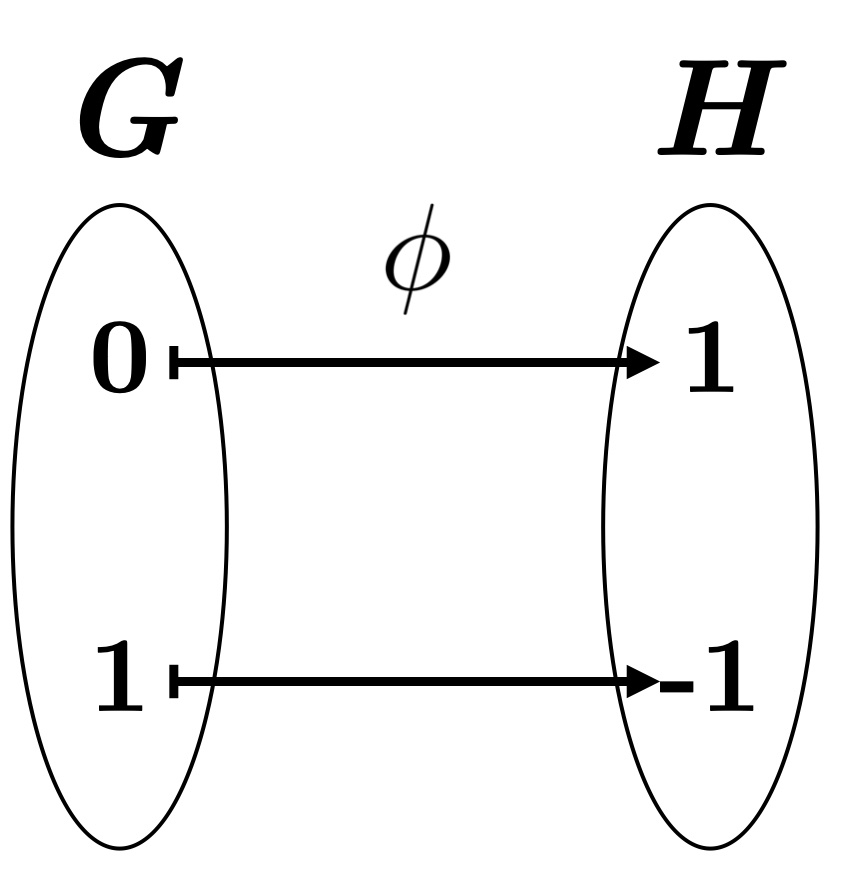
\includegraphics[width=2.5cm]{chapter4/Isomorphism Function Map.jpg}}
        \end{figure}
        \item $\phi$ is a homomorphism:\begin{itemize}
            \item $\phi(0\oplus_20) = \phi(0) = 1 = 1 \times 1 = \phi(0)\phi(0)$
            \item $\phi(0 \oplus_2 1) = \phi(1) = -1 = 1 \times (-1) = \phi(0)\phi(1)$
            \item $\phi(1 \oplus_2 0) = \phi(1) = -1 = (-1) \times 1 = \phi(1)\phi(0)$
            \item $\phi(1 \oplus_2 1) = \phi(0) = 1 = (-1) \times (-1) = \phi(1)\phi(1)$
        \end{itemize}
    \end{itemize}
    Thus $\phi$ is an isomorphism, which means $G \cong H$.
\end{example}

\begin{example}
    Let $S$ denote the set of positive real numbers. We show that $(\mathbb{R}, +) \cong (S, \times)$ by considering the map $\phi: \mathbb{R} \to S, x \mapsto e^x$.
    \begin{itemize}
        \item \textbf{Homomorphism}:
        \[
            \phi(x+y) = e^{x+y} = e^xe^y = \phi(x)\phi(y)
        \]

        \item \textbf{Injective}: Suppose $x$ and $y$ are elements in $\mathbb{R}$ such that $\phi(x) = \phi(y)$. Therefore $e^x = e^y$ which quickly implies $x = y$ by applying the natural logarithm ($\ln$) on both sides.

        \item \textbf{Surjective}: Suppose $y \in S$. Then $\ln y \in \mathbb{R}$, so $\phi(\ln y) = e^{\ln y} = y$, meaning every element in the codomain $S$ has a preimage.
    \end{itemize}

    Thus $\phi$ is an isomorphism, meaning that $(\mathbb{R}, +) \cong (S, \times)$.
\end{example}

\begin{exercise}
    Let the groups $G = (\{1, 2, 3, 4\}, \otimes_5)$ and $H = (\{1, 3, 7, 9\}, \otimes_{10})$.
    \begin{partquestions}{\roman*}
        \item Show that $G = \langle 3 \rangle$ and $H = \langle 7 \rangle$.
        \item Prove that $G \cong H$ by considering $\phi: G \to H, 3^k \mapsto 7^k$.
    \end{partquestions}
\end{exercise}

\section{Consequences of Isomorphisms}
Isomorphisms between groups means that the two groups \textit{share the same structure}, in a manner of speaking. We look at a theorem that showcases the sharing of some of these properties.
\begin{theorem}\label{thrm-isomorphism-consequences}
    Let $\phi: G \to H$ be an isomorphism between the groups $G$ and $H$. Then
    \begin{enumerate}
        \item $|G| = |H|$;
        \item $\phi^{-1}: H \to G$ is an isomorphism;
        \item if $G$ is abelian then so is $H$;
        \item if $G$ is cyclic then so is $H$; and
        \item if $G$ has a subgroup of order $n$, then so does $H$.
    \end{enumerate}
\end{theorem}

\newpage

\begin{proof}
    We prove each of these statements individually.
    \begin{enumerate}
        \item Follows immediately from properties of a bijective function.

        \item Since $\phi$ is an isomorphism, it is bijective, which means that $\phi^{-1}$ exists and is also bijective. All that remains is to show that $\phi^{-1}$ is a homomorphism.

        Let $u$ and $v$ be in $H$. Then, since $\phi$ is surjective, there exist elements $x$ and $y$ in $G$ such that $\phi(x) = u$ and $\phi(y) = v$. Hence,
        \begin{align*}
            \phi^{-1}(uv) &= \phi^{-1}\left(\phi(x)\phi(y)\right)\\
            &= \phi^{-1}\left(\phi(xy)\right) & (\phi \text{ is a homomorphism})\\
            &= xy\\
            &= \phi^{-1}(u) \phi^{-1}(v).
        \end{align*}
        Thus $\phi^{-1}$ is an isomorphism.

        \item Suppose $u$ and $v$ are in $H$. Let $x$ and $y$ be elements in $G$ such that $\phi(x) = u$ and $\phi(y) = v$. Thus
        \begin{align*}
            uv = &= \phi(x)\phi(y) \\
            &= \phi(xy)\\
            &= \phi(yx) & (G \text{ is abelian})\\
            &= \phi(y)\phi(x)\\
            &= vu
        \end{align*}
        which means that $uv = vu$. Hence $H$ is abelian.

        \item Suppose $u$ is in $H$. Let $x$ be in $G$ such that $\phi(x) = u$. Since $G$ is cyclic, suppose $g$ is the generator of $G$, so $x = g^n$ for some integer $n$. This means that
        \begin{align*}
            u &= \phi(x)\\
            &= \phi(g^n)\\
            &= \underbrace{\phi(g)\phi(g)\phi(g)\cdots\phi(g)}_{n \text{ times}}\\
            &= \left(\phi(g)\right)^n\\
            &\in \left\langle \phi(g) \right\rangle.
        \end{align*}
        Thus any element $u$ in $H$ is in $\left\langle \phi(g) \right\rangle$, meaning $H \subseteq \left\langle \phi(g) \right\rangle$.

        However, as $\phi(g) \in H$, thus $\left\langle \phi(g) \right\rangle \leq H$ which means that $\left\langle \phi(g) \right\rangle \subseteq H$. Therefore, we have $H \subseteq \left\langle \phi(g) \right\rangle$ and $\left\langle \phi(g) \right\rangle \subseteq H$ simultaneously, meaning $H = \left\langle \phi(g) \right\rangle$, i.e. $H$ is a cyclic group.

        \item Suppose $K \leq G$ with $|K| = n$. Consider the subgroup $\phi(K)$. By properties of homomorphism, $\phi(K) \leq H = \phi(G)$. Now by the first property, $|K| = |\phi(K)| = n$, meaning that there is a subgroup of $H$ with order $n$, namely the subgroup $\phi(K)$.
    \end{enumerate}

    This proves the theorem.
\end{proof}

\begin{exercise}
    Let $\phi: G \to H$ be an isomorphism between the groups $G$ and $H$. Show that if $G$ has a normal subgroup with order $k$, then $H$ also has a normal subgroup of order $k$.
\end{exercise}

\newpage

\section{Links to Cyclic Groups}
With the tool of isomorphisms under our belt, we can prove two important theorems regarding cyclic groups. Before that, however, we formally introduce the idea of infinite cyclic groups.
\begin{definition}
    An infinite cyclic group\index{cyclic group!infinite} $G$ generated by $g$ is denoted by $\langle g \rangle$ and has order $|G| = \infty$. So,
    \[
        G = \{\dots, g^{-2}, g^{-1}, e, g, g^2, \dots\}.
    \]
\end{definition}

For brevity, we also have notation regarding the integers under addition.
\begin{itemize}
    \item When we write $\mathbb{Z}_n$, we mean the group $(\mathbb{Z}_n, \oplus_n)$\index{integers under addition!modulo $n$}.
    \item When we write $\mathbb{Z}$, we mean the group $(\mathbb{Z}, +)$\index{integers under addition}.
\end{itemize}

\begin{theorem}
    If $G$ is an infinite cyclic group with generator $g$, then $G \cong \mathbb{Z}$.
\end{theorem}
\begin{proof}[Proof (see \cite{proofwiki_infinite-cyclic-group})]
    Consider $\phi: \mathbb{Z} \to G$ where $\phi(n) = g^n$. We prove that $\phi$ is an isomorphism.
    \begin{itemize}
        \item \textbf{Homomorphism}:
        \[
            \phi(m+n) = g^{m+n} = g^mg^n = \phi(m)\phi(n)
        \]

        \item \textbf{Injective}: Let $m$ and $n$ be integers such that $\phi(m) = \phi(n)$. Without loss of generality, assume that $m \leq n$. Since $\phi(m) = \phi(n)$ we have $g^m = g^n = g^mg^{n-m}$ which implies that $g^{n-m} = e$ by cancellation law.

        Seeking a contradiction, suppose $m < n$. Since $g^{n-m} = e$, so $|g|$ divides $n-m$ (\myref{problem-element-to-power-of-multiple-of-order-is-identity}). However, $g$ is a generator of $G$, which means that $|g| = |G| = \infty$ divides $n-m$, which is absurd and thus a contradiction. Therefore, $m = n$, so $\phi(m) = \phi(n)$ implies that $m = n$. Hence $\phi$ is injective.

        \item \textbf{Surjective}: Suppose $x \in G = \langle g\rangle$, so $x = g^n$ for some integer $n$. Then $\phi(n) = g^n = x$ which means that $x$ has a preimage of $n$. Hence $\phi$ is surjective.
    \end{itemize}

    Therefore, $\phi$ is an isomorphism which means $G \cong \mathbb{Z}$.
\end{proof}

\begin{theorem}\label{thrm-finite-cyclic-group-isomorphic-to-Zn}
    If $G$ is a finite cyclic group of order $n$ with generator $g$, then $G \cong \mathbb{Z}_n$.
\end{theorem}
\begin{proof}[Proof (cf. {\cite[\S 63]{clark_1984}})]
    Consider $\phi: \mathbb{Z}_n \to G$ such that $\phi(m) = g^m$. We prove that $\phi$ is an isomorphism.
    \begin{itemize}
        \item \textbf{Homomorphism}:
        \[
            \phi(l+m) = g^{l+m} = g^lg^m = \phi(l)\phi(m)
        \]

        \item \textbf{Injective}: Let $l$ and $m$ be integers such that $\phi(l) = \phi(m)$. Without loss of generality, assume that $l \leq m$. Since $\phi(l) = \phi(m)$ we have $g^l = g^m = g^lg^{m-l}$ which implies that $g^{m-l} = e$ by cancellation law. This means that $|g|$ divides $m-l$ by \myref{problem-element-to-power-of-multiple-of-order-is-identity}.

        By way of contradiction, assume $l < m$, which means $m - l \in \{1, 2,\dots, n-1\}$. Therefore $m-l \leq n - 1 < n$. But since $g$ is a generator of $G$, thus $|g| = |G| = n$. Therefore, we have $n$ dividing $m-l$, which is smaller than $n$, a contradiction. Thus $l = m$, meaning $\phi$ is injective.

        \item \textbf{Surjective}: Suppose $x \in G = \langle g\rangle$, so $x = g^m$ for some integer $m$ in $\mathbb{Z}_n$. Then $\phi(m) = g^m = x$ which means that $x$ has a preimage of $m$. Hence $\phi$ is surjective.
    \end{itemize}

    Therefore, $\phi$ is an isomorphism which means $G \cong \mathbb{Z}_n$.
\end{proof}

In summary:
\begin{itemize}
    \item All cyclic groups with \textbf{infinite} order are isomorphic to the group of integers under addition, $\mathbb{Z}$.
    \item All cyclic groups with \textbf{finite} order $n$ are isomorphic to the group of integers under addition modulo $n$, $\mathbb{Z}_n$.
\end{itemize}

\begin{exercise}
    Let $G = (\{1, 3, 7, 9\}, \otimes_{10})$ be a group. Show that $G \cong \mathbb{Z}_n$ for some integer $n$.
\end{exercise}

\newpage

\section{Problems}
\begin{problem}
    Let $G$ be a group and $g \in G$. Define the map $f: G \to G, x \mapsto gxg^{-1}$. Prove that $f$ is an isomorphism.
\end{problem}

\begin{problem}
    Let $\mathbb{Q}_{>0}$ denote the set of positive rational numbers. Let $G = (\mathbb{Q}, +)$ and $H = (\mathbb{Q}_{>0}, \times)$ be groups. Prove that $G \not\cong H$.
\end{problem}

\begin{problem}
    Let $G$ and $H$ \textbf{both} be the additive group of integers. Define a map $\phi: G \to H$ such that $\phi(n) = 2n$.
    \begin{partquestions}{\alph*}
        \item Prove that $\phi$ is a homomorphism.
        \item Prove that $\phi$ is injective.
        \item Prove that there does \textbf{not} exist a homomorphism $\psi: H \to G$ such that $\psi(\phi(n)) = n$.
    \end{partquestions}
\end{problem}

\begin{problem}
    Let $G$ be a group. Define a map $f: G \to G$ such that $f(g) = g^{-1}$ for all $g$ in $G$. Prove that $G$ is abelian if and only if $f$ is a homomorphism.
\end{problem}

\begin{problem}
    Let $G$ and $H$ be groups. Suppose that we have a surjective homomorphism $\phi: G \to H$. Prove that if $G$ is abelian, then so is $H$.
\end{problem}

\begin{problem}
    Let $G$ and $H$ be groups. Suppose that we have a surjective homomorphism $\phi: G \to H$. Let $N \unlhd G$. Show that $\phi(N) \unlhd H$.\newline
    (That is, the image of $N$ under $\phi$ is a normal subgroup of $H$.)
\end{problem}

\newpage

\begin{problem}\label{problem-Zn-isomorphic-to-Z-by-nZ}
    Let $G = (\mathbb{Z}_n, \oplus_n)$, and $H = \mathbb{Z}/(n\mathbb{Z})$ be under addition. Prove that $G \cong H$.
\end{problem}
\begin{remark}
    Whenever we are dealing with homomorphisms involving $(\mathbb{Z}_n, \oplus_n)$, it is usually easier to replace it with $\mathbb{Z}/(n\mathbb{Z})$ and do the homomorphism that way.
\end{remark}

\begin{problem}\label{problem-subgroup-of-quotient-group-is-quotient-group}
    Let $G$ be a group and $N \unlhd G$. Let $B$ be a subgroup of the quotient group $G/N$. Prove that $B = A/N$, where $A$ is a subgroup of $G$ such that $N \subseteq A$.
\end{problem}
